\documentclass[10pt]{article}
%%%%%%%%%%%%%%%%%%%%%%%%%%%%%%%%%%%%%%%%
\usepackage{amsmath}
\usepackage{verbatim}
\usepackage[usenames,dvipsnames]{color}
\usepackage{ulem}
\usepackage{setspace}
\usepackage{lscape}
\usepackage{longtable}
\usepackage[top=1.25in,bottom=1.5in,left=1in,right=1.5in,landscape]{geometry}
\usepackage{graphicx}
\usepackage{epstopdf}
\usepackage[usenames,dvipsnames]{pstricks}
\usepackage{epsfig}
\usepackage{pstricks-add}
\usepackage{pst-node}
\usepackage{fancyhdr}
\usepackage[absolute,showboxes]{textpos}

%TCIDATA{OutputFilter=LATEX.DLL}
%TCIDATA{Version=5.00.0.2552}
%TCIDATA{<META NAME="SaveForMode" CONTENT="1">}
%TCIDATA{Created=Thursday, August 28, 2003 13:38:44}
%TCIDATA{LastRevised=Thursday, August 14, 2008 15:20:27}
%TCIDATA{<META NAME="GraphicsSave" CONTENT="32">}
%TCIDATA{<META NAME="DocumentShell" CONTENT="Standard LaTeX\Blank - Standard LaTeX Article">}
%TCIDATA{Language=American English}
%TCIDATA{CSTFile=LaTeX article (bright).cst}

\setcounter{MaxMatrixCols}{10}

\newenvironment{proof}[1][Proof]{\noindent\textbf{#1.} }{\ \rule{0.5em}{0.5em}}
\setlength{\columnsep}{.2in}

\renewcommand{\labelitemii}{$\cdot$}

\pagestyle{fancy} \fancyhead{} \fancyfoot{} \rfoot{} \lfoot{}

\newcommand{\slide}[2]{
\begin{textblock}{11}(0,0)
\textcolor{Black}{\textbf{\huge \rule{0pt}{1in} \raisebox{.2in}{#1}}}
\end{textblock}
\begin{Large} \noindent
#2
\end{Large}
\vfill \pagebreak}

\setlength{\TPHorizModule}{1in}
\setlength{\TPVertModule}{1in}
\textblockcolour{Yellow}
\renewcommand{\headrulewidth}{0pt}



\begin{document}
\onehalfspacing 

\lfoot{The Solow Model} \rfoot{Economic Growth}

\slide{Production}{Real output, $Y$, is produced according to a function like this
\begin{equation}
Y = F(K,L)
\end{equation}
where $K$ is the stock of physical capital and $L$ is the number of workers.

\vspace{.25in}\noindent Very often, we use a very specific function, $F()$, called the Cobb-Douglas.
\begin{equation}
Y = K^{\alpha} L^{1-\alpha}
\end{equation}

\vspace{.25in}\noindent The Cobb-Douglas has \textbf{constant returns to scale}; if you double the amount of each input, you double output. 
\begin{equation}
(zK)^{\alpha} (zL)^{1-\alpha} = z^{\alpha}z^{1-\alpha}K^{\alpha} L^{1-\alpha} = z K^{\alpha} L^{1-\alpha} = zY
\end{equation}
}

\slide{Firms}{We assume that firms are perfectly competitive
\begin{itemize}
	\item There are many firms, all producing the same homogeous output
	\item Firms enter and exit freely
	\item They all produce using a similar Cobb-Douglas function
	\item They are all price-takers for the use of labor and capital
\end{itemize}

\vspace{.25in}\noindent For the representative firm, profits are
\begin{equation}
\Pi = K^{\alpha}L^{1-\alpha} - rK - wL
\end{equation}
where $r$ is the market rate for renting capital and $w$ is the wage of a worker.

\vspace{.25in}\noindent The firm's profit-maximizing decision (first-order conditions) are
\begin{eqnarray}
MPL = (1-\alpha)\frac{Y}{L} &=& w \\
MPK = \alpha\frac{Y}{K} &=& r
\end{eqnarray}
which just say that the firm sets the marginal product of a factor equal to its marginal cost.
}

\slide{Factor Income}{From the firm first-order conditions
\begin{eqnarray}
MPL = (1-\alpha)\frac{Y}{L} &=& w \\
MPK = \alpha\frac{Y}{K} &=& r
\end{eqnarray}
note that total payments to factors are equal to total output
\begin{equation}
wL + rK = (1-\alpha)\frac{Y}{L}L + \alpha\frac{Y}{K}K = (1-\alpha)Y + \alpha Y = Y.
\end{equation}
This means that firms all have zero profits
\begin{equation}
\Pi = Y - rK - wL = 0.
\end{equation}
This is consistent with our assumption that firms are perfectly competitive with each other, and firms enter and exit freely. If there were profits, more firms would enter and compete them away.
}

\slide{Factor Shares}{Calculate the fraction of total output that is paid to each factor.
\begin{equation}
\frac{wL}{Y} = (1-\alpha)\frac{Y}{L} \frac{L}{Y} = (1-\alpha)
\end{equation}
and 
\begin{equation}
\frac{rK}{Y} = \alpha \frac{Y}{K} \frac{K}{Y} = \alpha
\end{equation}

\vspace{.25in}\noindent Factor shares of output are thus constant when we use the Cobb-Douglas, regardless of the amount of $K$ or $L$. Consistent with the stylized facts on factor shares. Those facts suggest that $\alpha = 1/3$ and $(1-\alpha) = 2/3$, roughly.

}

\slide{Output per Worker}{We typically care about output \textit{per worker}, not just total output. Divide total output by $L$ to get
\begin{equation}
y = \frac{Y}{L} = \frac{K^{\alpha}L^{1-\alpha}}{L} = \frac{K^{\alpha}}{L^{\alpha}} = k^{\alpha}
\end{equation}
where we are using $y = Y/L$ and $k = K/L$ to represent per-worker values.

\vspace{.25in}\noindent Captial per worker has a diminishing marginal output. If $k$ rises, output per worker rises, but the size of the increase falls as $k$ increases.

\begin{center}
\scalebox{1}{
\begin{pspicture}(10,9)
\psline{->}(0,0)(9,0) \psline{->}(0,0)(0,8) \pscurve[linewidth=3pt](0,0)(4,6)(9,7) \rput(9.3,0){$k$} \rput(0,8.3){$y$} \rput(9,6.3){$y=k^{\alpha}$}
\end{pspicture}
}
\end{center}

}

\slide{Capital Accumulation}{Output depends on capital and labor, so we need to know how those two things accumulate over time. Start with capital. 
\begin{equation}
\dot{K} = sY - \delta K
\end{equation}

\vspace{.25in}\noindent $\dot{K}$ is the \textit{change} in the capital stock. It is the continuous time version of $K_{t+1} - K_t$. 

\vspace{.25in}\noindent $sY$ is gross investment. We know that total income ($wL+rK$) is equal to total output ($Y$). We assume that individuals - who work and own the capital - save a constant fraction, $0<s<1$, of their income.

\vspace{.25in}\noindent $\delta K$ is depreciation. A fixed fraction, $0<\delta<1$, of the existing capital stock, $K$, breaks down at any given moment. 

\vspace{.25in}\noindent It will be useful to write this as the \textit{growth rate} of capital, or divide through by $K$,
\begin{equation}
\frac{\dot{K}}{K} = s\frac{Y}{K} - \delta.
\end{equation}
}

\slide{Capital per Worker Accumulation}{What happens to capital \textit{per worker}? To analyze this, we will use some mathematical tools reviewed previously - take logs and derivatives.
\begin{eqnarray}
k &=& \frac{K}{L} \\
\ln{k} &=& \ln{K} - \ln{L} \\
\frac{\partial}{\partial t} \ln{k} &=& \frac{\partial}{\partial t}\ln{K} - \frac{\partial}{\partial t} \ln{L} \\
\frac{\dot{k}}{k} &=& \frac{\dot{K}}{K} - \frac{\dot{L}}{L} 
\end{eqnarray}

\vspace{.25in}\noindent From the prior slide, we know that 
\begin{equation}
\frac{\dot{K}}{K} = s\frac{Y}{K} - \delta
\end{equation}
so 
\begin{equation}
\frac{\dot{k}}{k} = s\frac{Y}{K} - \delta - \frac{\dot{L}}{L}.
\end{equation}
}

\slide{Population Growth}{The last piece of information we need is the growth rate of the number of workers, $\dot{L}/L$. We assume that the number of workers grows at the same rate as the population. Let
\begin{equation}
L(t) = L(0)e^{nt}
\end{equation}
or the number of workers exhibits exponential growth. 

\vspace{.25in}\noindent The growth rate of the number of workers is thus
\begin{equation}
\frac{\dot{L}}{L} = n,
\end{equation}
which you can find by taking logs and derivatives of the equation for $L(t)$.
}

\slide{The Solow Equation}{Plugging in the growth rate of workers we now have
\begin{equation}
\frac{\dot{k}}{k} = s\frac{Y}{K} - \delta - n.
\end{equation}
which says the growth rate of capital per worker depends on the capital/output ratio ($K/Y$) and the parameters $s$, $\delta$, and $n$.

\vspace{.25in}\noindent We can re-write this into what is commonly called \textit{the Solow Equation},
\begin{eqnarray}
\frac{\dot{k}}{k} &=& s\frac{Y/L}{K/L} - \delta - n \\
 &=& s \frac{y}{k} - \delta - n.
\end{eqnarray}
and then multiply both sides by $k$ to get
\begin{equation}
\dot{k} = sy - (\delta+n)k.
\end{equation}

\vspace{.25in}\noindent Finally, recall that we can write output per worker in terms of capital per worker, $y = k^{\alpha}$, so that we have
\begin{equation}
\dot{k} = s k^{\alpha} - (\delta+n)k
\end{equation}
}

\slide{Solving the Model}{First, what do we mean by ``solve''? We mean that we want to be able to express the endogenous variables in terms of \textit{only} exogenous ones. 

\vspace{.25in}\noindent Endogenous variables - things we are trying to explain
\begin{itemize}
	\item Output $Y$ and/or output per worker $y$
	\item Capital $K$ and/or capital per worker $k$
\end{itemize}

\vspace{.25in}\noindent Exogenous variables - things we take as given
\begin{itemize}
	\item $\alpha$, capital's share in output
	\item $s$, the savings rate
	\item $n$, the population growth rate
	\item $\delta$, the depreciation rate
	\item $k_0$, the initial level of capital per worker
\end{itemize}
}

\slide{Solve the Solow Model}{Getting a precise equation for $k$ or $y$ is not terribly easy. However, we can see the solution in some simple diagrams.
\begin{center}
\scalebox{1.3}{
\begin{pspicture}(10,9)
\psline{->}(0,0)(9,0) \psline{->}(0,0)(0,8) \pscurve[linewidth=3pt](0,0)(3,4)(9,6) \rput(9.3,0){$k$} \rput(9.4,6){$sk^{\alpha}$} \psline[linewidth=3pt](0,0)(9,7) \rput(9,7.3){$(\delta+n)k$} \psline[linestyle=dotted](7.2,0)(7.2,5.5) \rput(7.2,-.3){$k^{\ast}$} \psline[ArrowInside=->,ArrowInsideNo=5,arrowsize=.3,ArrowInsideOffset=0.1](0,0)(7.2,0)
\psline[ArrowInside=->,ArrowInsideNo=1,arrowsize=.3,ArrowInsideOffset=0.1](9,0)(7.2,0)
\end{pspicture}
}
\end{center}

}

\slide{Implications}{The diagram shows us that
\begin{itemize}
	\item If $k < k^{\ast}$, then $sk^{\alpha} > (\delta+n)k$, and $\dot{k} > 0$
	\item If $k > k^{\ast}$, then $sk^{\alpha} < (\delta+n)k$, and $\dot{k} < 0$
\end{itemize}

\vspace{.25in}\noindent The Solow model predicts that capital per worker will stabilize at some value $k^{\ast}$ where investment $sk^{\alpha}$ just offsets depreciation and population growth $(\delta+n)k$. We refer to $k^{\ast}$ as the \textit{steady state} of the Solow Model.

\vspace{.25in}\noindent We have solved the Solow model in a general sense. If you tell me $k_0$, the initial starting point for capital per worker, and the parameters $\alpha$, $s$, $n$, and $\delta$, I can tell you whether capital per worker will grow or shrink.
\begin{itemize}
	\item $\alpha$, $s$, $n$, and $\delta$ describe the two lines
	\item $k_0$ tells me where along the x-axis I start
\end{itemize}
}

\slide{The Steady State}{No matter what, $k$ eventually ends up at $k^{\ast}$. We can give a precise answer to what determines $k^{ast}$. It is the value of $k$ such that $\dot{k}=0$. Or
\begin{equation}
0 = s k^{\alpha} - (\delta+n)k.
\end{equation}
This solves to
\begin{eqnarray}
 (\delta+n)k  &=& s k^{\alpha}\\
k^{1-\alpha} &=&  \frac{s}{\delta+n}\\
k  &=&  \left(\frac{s}{\delta+n}\right)^{1/(1-\alpha)} 
\end{eqnarray}
which is the capital per worker at steady state, or
\begin{equation}
k^{\ast} = \left(\frac{s}{\delta+n}\right)^{1/(1-\alpha)} 
\end{equation}
}

\slide{Implications}{The steady state is
\begin{equation}
k^{\ast} = \left(\frac{s}{\delta+n}\right)^{1/(1-\alpha)} 
\end{equation}
which depends only on the parameters of the model. Note that it does \textit{not} depend on $k_0$.

\vspace{.25in}\noindent This implies that
\begin{itemize}
	\item $k^{\ast}$ (and so $y^{\ast}$) is rising with the savings rate, $s$
	\item $k^{\ast}$ (and so $y^{\ast}$) is declining with the population growth rate, $n$
\end{itemize}
}

\slide{Savings and Output per Worker}{
\begin{center}
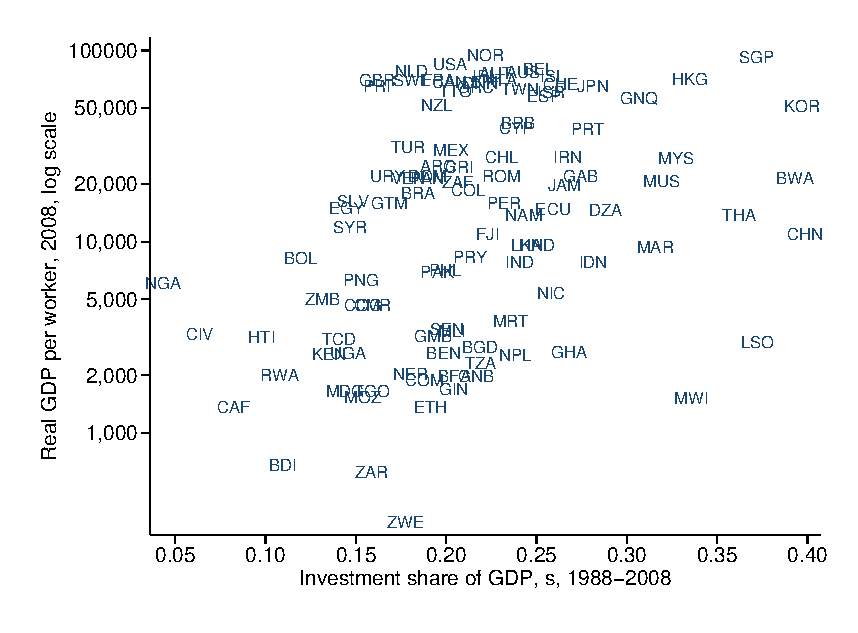
\includegraphics[scale=1.3]{figure_2_6.eps}
\end{center}
}

\slide{Savings and Output per Worker}{
\begin{center}
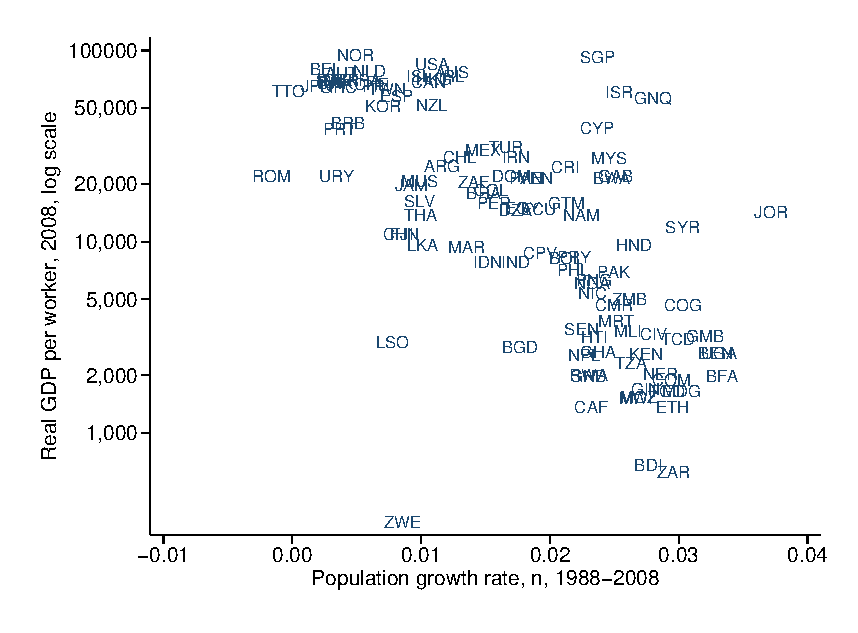
\includegraphics[scale=1.3]{figure_2_7.eps}
\end{center}
}

\slide{Statics}{What if the savings rate, $s$, changes? Could be a policy change, or some difference in individuals willingness to save for the future. Let $s$ go to $s' > s$. 
\begin{center}
\scalebox{1.3}{
\begin{pspicture}(10,9)
\psline{->}(0,0)(9,0) \psline{->}(0,0)(0,8) \pscurve[linewidth=3pt](0,0)(3,4)(9,6) \rput(9.3,0){$k$} \rput(9.5,6){$s'k^{\alpha}$} \psline[linewidth=3pt](0,0)(9,7) \rput(9,7.3){$(\delta+n)k$} \psline[linestyle=dotted](7.2,0)(7.2,5.5) \rput(7.2,-.3){$k^{\ast\ast}$} \pscurve[linewidth=2pt,linecolor=gray](0,0)(2,2.3)(4,3.1)(9,3.6) \psline[linestyle=dotted](4,0)(4,3.1)
\rput(9.4,3.6){$sk^{\alpha}$} \rput(4,-.3){$k^{\ast}$}
\psline[ArrowInside=->,ArrowInsideNo=4,arrowsize=.3,ArrowInsideOffset=0.1](4,0)(7.2,0)
\psline{->}(9,4)(9,5.7)
\end{pspicture}
}
\end{center}
}

\slide{Savings Increase}{What is the effect of $s$ rising to $s'$?
\begin{itemize}
	\item The steady state rises to $k^{\ast\ast}$. The economy will be richer \textit{eventually}
	\item Immediately after the change, $k<k^{\ast\ast}$, so $\dot{k}>0$, capital starts growing
	\item Output per worker grows until the economy reaches the new steady state
\end{itemize}
\begin{center}
\scalebox{1.1}{
\begin{pspicture}(10,9)
\psline{->}(0,0)(9,0) \psline{->}(0,0)(0,8) \psline[linewidth=2pt](0,2)(2,2) \pscurve[linewidth=2pt](2,2)(3,3.5)(4,4)(9,4.4) \rput(0,8.3){$y$} \rput(-.4,2){$y^{\ast}$} \rput(-.4,4.4){$y^{\ast\ast}$} \psline[linestyle=dotted](0,4.4)(9,4.4) \rput(9.5,0){$Time$}
\psline[linestyle=dotted](2,0)(2,2) \rput(2,-.3){$s$ changes to $s'$}
\end{pspicture}
}
\end{center}
}

\slide{Growth Rates}{The Solow model predicts that growth is faster, the farther away from steady state is an economy. Look at the growth rate of $k$
\begin{equation}
\frac{\dot{k}}{k} = \frac{s}{k^{1-\alpha}} - (\delta + n).
\end{equation}
As $k$ rises, the growth rate of $k$ falls.
\begin{center}
\scalebox{1.1}{
\begin{pspicture}(10,9)
\psline{->}(0,0)(9,0) \psline{->}(0,0)(0,8) \psline[linewidth=2pt](0,4)(9,4) \rput(9.6,4){$\delta +n$}
\pscurve[linewidth=2pt](1,8)(5,4)(9,2) \rput(9,1.6){$s/k^{1-\alpha}$} \rput(9.3,0){$k$} \psline[linestyle=dotted](5,4)(5,0) \rput(5,-.3){$k^{\ast}$} \psline{<->}(2,4.1)(2,6.5) \rput(1.5,5.3){$\dot{k}/k$}
\end{pspicture}
}
\end{center}
}

\slide{Trend Growth}{Growth rates go to zero in the Solow model. $y$ does not grow in steady state. To see this, take logs and derivatives of $y = k^{\alpha}$ to find
\begin{eqnarray}
\ln{y} &=& \alpha \ln{k} \\
\frac{\dot{y}}{y} = \alpha \frac{\dot{k}}{k}.
\end{eqnarray}
Because $\dot{k} = 0$ in steady state, it must be that $\dot{y}/y = 0$ in steady state.

\vspace{.25in}\noindent To allow for trend growth in the Solow model, we'll incorporate productivity improvements. Let production be
\begin{equation}
Y = K^{\alpha}(AL)^{1-\alpha}
\end{equation}
where $A$ is labor-augmenting technological progress. In per worker terms this is
\begin{equation}
y = k^{\alpha} A^{1-\alpha}
\end{equation}

\vspace{.25in}\noindent Growth in $A$ will allow there to be trend growth in output per worker even in steady state.
}

\slide{Exogenous Technological Change}{We assume that
\begin{equation}
A(t) = A(0)e^{gt}
\end{equation}
which implies that
\begin{equation}
\frac{\dot{A}}{A} = g.
\end{equation}
}

\slide{Trend Growth}{We can also rconsider growth in output per worker. Take logs and derivatives of $y = k^{\alpha} A^{1-\alpha}$ to get
\begin{equation}
\frac{\dot{y}}{y} = \alpha \frac{\dot{k}}{k} + (1-\alpha)\frac{\dot{A}}{A}.
\end{equation}

\vspace{.25in}\noindent We're looking for the situation when $\dot{y}/y$ is constant. This requires $\dot{k}/k$ to be constant. From
\begin{equation}
\frac{\dot{k}}{k} = s \frac{y}{k} - (\delta +n)
\end{equation}
capital per worker growth will be constant only if $y/k$ is constant. $y/k$ will be constant only if $\dot{y}/y = \dot{k}/k$. 

\vspace{.25in}\noindent Putting this all together
\begin{eqnarray}
\frac{\dot{y}}{y} &=& \alpha \frac{\dot{y}}{y} + (1-\alpha)g \\
\frac{\dot{y}}{y} &=& g
\end{eqnarray}
or $y$ must grow at rate $g$ if it is going to grow at a constant rate.
}

\slide{Balanced Growth Path}{The steady state of the Solow model will be exactly a situation where growth in $y$ is constant at $g$. Further, $y$ and $k$ and $A$ will all grow at the same rate. The Solow model produces a \textit{balanced growth path} where everything's growth rate remains constant.

\vspace{.25in}\noindent What is the steady state when there is technology? We saw above that $\dot{y}/y = g$ is the constant growth rate. This also implies $\dot{k}/k = g$. So in steady state 
\begin{equation}
g = s \frac{y}{k} - (\delta +n).
\end{equation}
Plug in for $y$ to get
\begin{equation}
g = s \frac{A^{1-\alpha}}{k^{1-\alpha}} - (\delta+n).
\end{equation}
Solve for
\begin{equation}
\frac{k}{A} = \left(\frac{s}{\delta +n +g} \right)^{1/(1-\alpha)}.
\end{equation}

}

\slide{Steady State with Technology}{We said that
\begin{equation}
\frac{k}{A} = \left(\frac{s}{\delta +n +g} \right)^{1/(1-\alpha)}
\end{equation}
in steady state. The ratio $k/A$ is constant because $k$ and $A$ grow at the rate $g$.

\vspace{.25in}\noindent Output per worker in this steady state is
\begin{eqnarray}
y &=& k^{\alpha} A^{1-\alpha} \\ 
&=& A \left(\frac{k}{A}\right)^{\alpha} \\
&=& A \left(\frac{s}{\delta +n +g} \right)^{\alpha/(1-\alpha)} \\
y(t) &=& A(t) \left(\frac{s}{\delta +n +g} \right)^{\alpha/(1-\alpha)}
\end{eqnarray}
where the $y(t)$ and $A(t)$ are there to be explicit that both are growing over time. 
}

\slide{Level Effects versus Growth Effects}{
\begin{equation}
y(t) = A(t) \left(\frac{s}{\delta +n +g} \right)^{1/(1-\alpha)}
\end{equation}
The growth rate of $y$ is equal to $g$ along the balanced growth path - which is the steady state of the Solow model. But the \textit{level} of $y$ depends on the term in the parentheses.

\vspace{.25in}\noindent The parameters for savings, $s$, and population growth, $n$, have effects on the level of output per worker, but don't alter the \textit{growth rate} of output per worker.

\vspace{.25in}\noindent Changes in those parameters will induce a temporary surge (or decline) in growth relative to $g$ as the economy shifts to the new trend line.
}

\slide{Example}{Consider an increase in savings from $s$ to $s'$. You can use the old Solow model without technology to consider what happens in the transition -- output per worker grows rapidly for a while until we reach the new steady state. Then just add trend growth.

\begin{center}
\scalebox{1.1}{
\begin{pspicture}(10,9)
\psline{->}(0,0)(9,0) \psline{->}(0,0)(0,8) \psline[linewidth=2pt](0,2)(2,3) \pscurve[linewidth=2pt](2,3)(3,4.4)(4,5)(9,7.6) \rput(0,8.3){$y$} \rput(9.6,0){$Time$}
\psline[linestyle=dotted](2,0)(2,3) \rput(2,-.3){$s$ changes to $s'$} \psline[linestyle=dotted](0,2)(9,6.5)
\end{pspicture}
}
\end{center}

}


\end{document}